\section*{Цель работы.}
Изучение работы с функциями в математическом пакете MatLab.

\section*{Задания.}
\begin{enumerate}
    \item Создать функцию в соответствии с \cref{fig:source}. Сделать ее нечетной (посколько график \cref{fig:source} проходит через точку $(0, 0)$).
    \item Создать прототип функции, сохраняющей внешний вид рисунка из \cref{fig:source}, но с произвольными числами, с учетом нечетности.
    \item Создать функции для выполнения операций из \cref{table:source}, но с произвольными матрицами. Добавить в функции вариативность действий (сумма/произведение).
    \item Создать скрипт для вызова функций из п. 1-3 и вывода результатов.
\end{enumerate}

\section*{Требования к выполнению заданий.}
\begin{enumerate}
    \item Для выполнения п. 2 нужно создать функцию, возвращающую объект типа \textit{function\_handle}.
    \item Функция для поиска максимальных/минимальных элементов должна быть адаптирована к разному количеству выходных аргументов, и уметь возвращать сам элемент/строку/столбец, и его индекс/номер.
    \item Функция для вычисления частных сумм/произведений должна иметь дополнительный входной символьный аргумент: если символ \mintinline{x}!‘s’! --- нужно считать сумму, если \mintinline{x}!‘p’! --- произведение.
    \item Вычисление сумм и произведений должно быть реализовано в виде локальных функций.
\end{enumerate}

\begin{figure}[b]
    \centering
    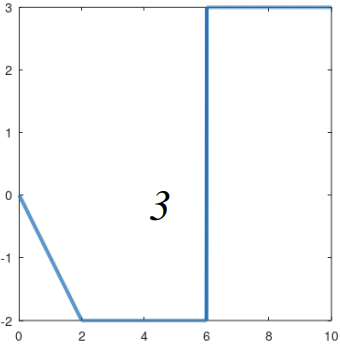
\includegraphics[width=0.4\textwidth]{figs/source.png}
    \caption{Исходный график кусочно-линейной функции}
    \label{fig:source}
\end{figure}

\section*{Экспериментальные результаты.}
\subsection*{ \boxed{\text{ Задание 1. }} }

\begin{quote}
    \textit{Создать функцию в соответствии с \cref{fig:source}. Сделать ее нечетной (посколько график \cref{fig:source} проходит через точку $(0, 0)$). }
\end{quote}

\begin{listing}[H]
    \caption{Нечетный вариант функции из \cref{fig:source}}
    \label{lst:ex1.m}
    \inputminted[
        % firstline      = 1,
        % lastline       = 10,
        % highlightlines = {1-10},
    ]{matlab}{code/ex1.m}
\end{listing}

В данном задании используется функция \textit{fliprl}, суть которой заключается в отражении массива по горизонтали. Так, если у нас есть массив $A = [1, 2, 3]$, то применение функции \textit{fliprl} даст нам $fliprl(A) = [3, 2, 1]$.
В совокупности с домножением на $-1$, это позволяет нам получить отрицательные значения функции для отрицательных значений $x$, что и требуется для построения нечетной функции.

В заключение отраженная и исходная части функции объединяются в один массив, при этом исключается повторяющаяся точка в начале координат (нулевой элемент).
Примечательно, что для построения корректно выглядящего графика, необходимо использовать достаточно мелкий шаг для $x$ (в данном случае $0.01$).


\subsection*{ \boxed{\text{ Задание 2. }} }
\begin{quote}
    \textit{Создать прототип функции, сохраняющей внешний вид рисунка из \cref{fig:source}, но с произвольными числами, с учетом нечетности.}
\end{quote}

\begin{table}[hb]
    \centering
    \renewcommand{\arraystretch}{2.5}
    \caption{Исходные данные для варианта 3}
    \label{table:source}
    \begin{tabularx}{\linewidth}{cCC}
        Исходные данные & Результат поиска & Результат вычисления \\
        \toprule

        $$
            \begin{bmatrix}
                -1.1 & 4    & -11 & 6    \\
                3    & 0    & 5   & 2.3  \\
                6.2  & -0.3 & 3   & -6.4
            \end{bmatrix}
        $$
        & столбец с минимальным элементом & накопительная сумма элементов столбцов \\
    \end{tabularx}
\end{table}

\begin{listing}[H]
    \caption{Прототип функции}
    \label{lst:ex2.m}
    \inputminted[
        % firstline      = 1,
        % lastline       = 10,
        % highlightlines = {1-10},
    ]{matlab}{code/ex2.m}
\end{listing}

Реализация задания 1 в функции для задания 2 заключается в параметризации всех констант, которые определяют вид функции.
Были добавлены параметры для интервалов разрывов функции $a$ и $b$ (точки $(2, -2)$ и $(6,-2)$ соотв. на \cref{fig:source}), коэффициента наклона линейного участка $k$ (промежуток $x\in[0; 2]$ на \cref{fig:source}), а также значений горизонтальных участков $m$ и $n$ (промежутки $[2; 6]$ и $[6; 8]$ на \cref{fig:source}).
Это позволяет вызывать функцию с любыми значениями этих параметров, сохраняя при этом общий вид функции, представленный на \cref{fig:source}.


\subsection*{ \boxed{\text{ Задание 3. }} }
\begin{quote}
    \textit{Создать функции для выполнения операций из \cref{table:source}, но с произвольными матрицами. Добавить в функции вариативность действий (сумма/произведение).}
\end{quote}

\begin{codemultipage}
    \captionof{listing}{Функция для выполнения разл. операций над произв. матрицей\label{lst:ex3.m}}
    \inputminted{matlab}{code/ex3.m}
\end{codemultipage}

Для создания данной функции за основу были взяты наработки из предыдущих лабораторных работ.
Данная функция принимает на вход матрицу и два символьных аргумента: режим поиска (максимальный или минимальный элемент) и режим накопительной суммы или произведения.

Вначале функция проверяет корректность входных данных, чтобы избежать ошибок при выполнении. Затем, в зависимости от указанных режимов, выполняются соответствующие операции.

Для нахождения максимальных или минимальных элементов используется перебор всех элементов в матрице. В качестве более эффективной альтернативы можно использовать встроенные функции MatLab, такие как \mintinline{x}!max! и \mintinline{x}!min!, которые оптимизированы для работы с матрицами. Однако важно также вернуть индексы найденных элементов, поэтому в данном случае используется простой перебор для простоты реализации алгоритма.

Аналогично, для вычисления накопительных сумм или произведений используются уже известные алгоритмы из предыдущих лабораторных работ.

\subsection*{ \boxed{\text{ Задание 4. }} }
\begin{quote}
    \textit{Создать скрипт для вызова функций из п. 1-3 и вывода результатов.}
\end{quote}

\begin{codemultipage}
    \captionof{listing}{Скрипт для работы с функциями\label{lst:ex4.m}}
    \inputminted{matlab}{code/ex4.m}
\end{codemultipage}

В данном скрипте под функцией \mintinline{x}!ex3! понимается функция из задания 3, а под \mintinline{x}!ex2! --- функция из задания 2.
Алгоритм запрашивает входные параметры для функций у пользователя, вызывает функции с этими параметрами, а затем выводит результаты на экран.

\section*{Выводы.}

Алгоритм работает исправно и корректно выполняет все поставленные задачи (см. \cref{fig:result.png}).

\begin{figure}[hbt]
    \centering
    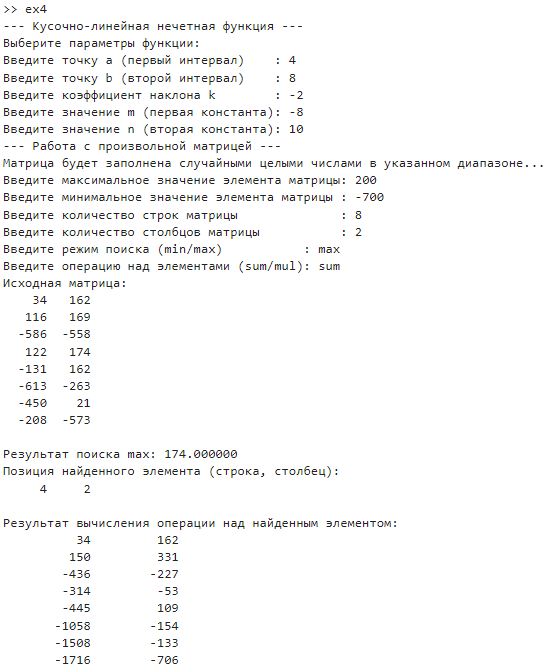
\includegraphics[width=0.8\textwidth]{figs/result.png}
    \caption{Вызов программы}
    \label{fig:result.png}
\end{figure}

\begin{figure}[hb]
    \centering
    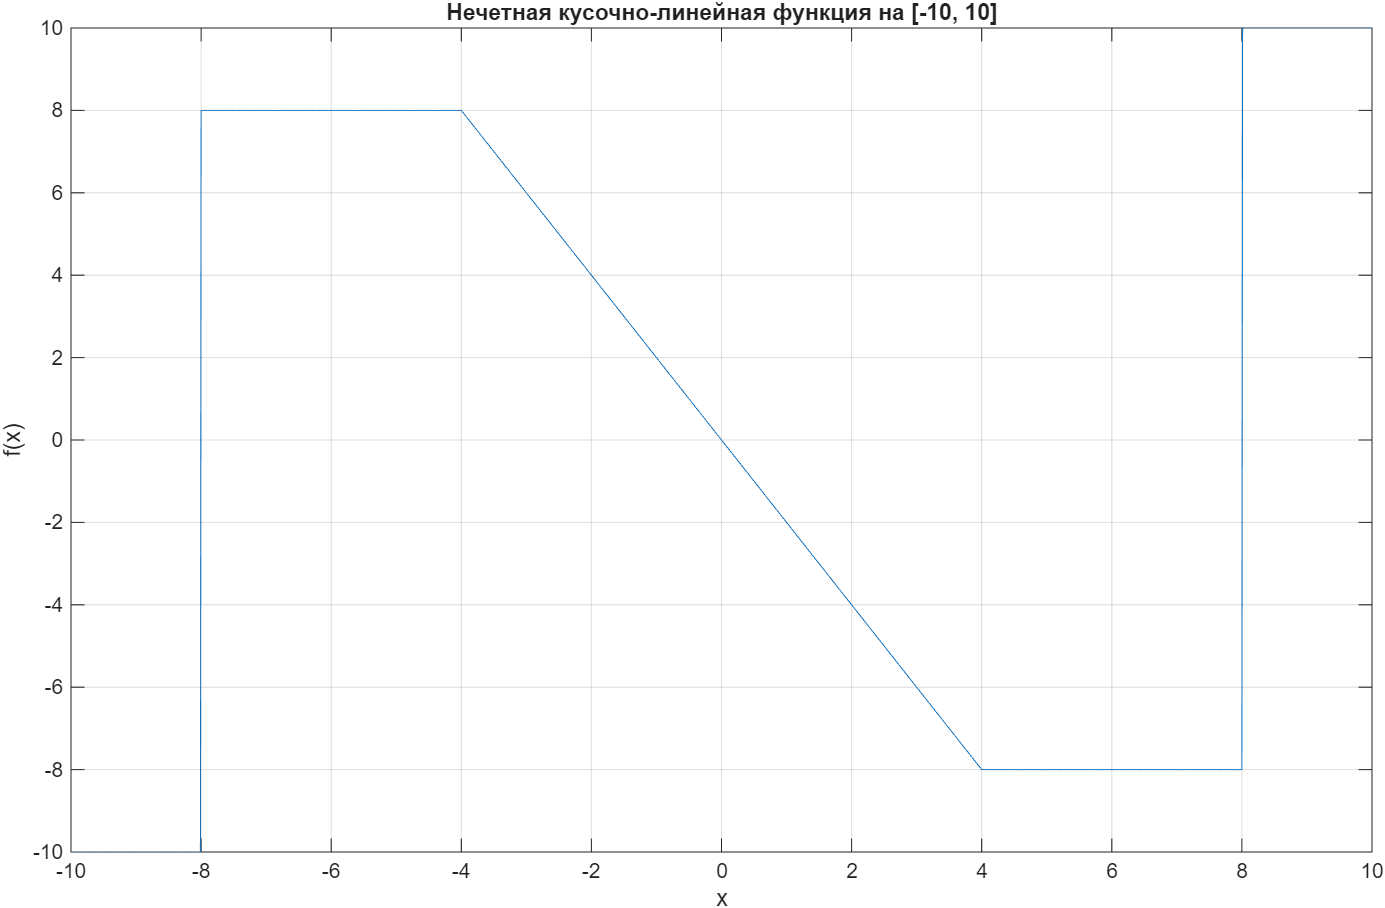
\includegraphics[width=0.8\textwidth]{figs/result_figure.png}
    \caption{График при параметрах из \cref{fig:result.png}}
    \label{fig:result_figure.png}
\end{figure}

Были решены все задачи. Цель лабораторной работы была успешно достигнута, продемонстрировав владение всеми необходимыми знаниями для работы с функциями в MatLab.